%%%%%%%%%%%%%%%%%%%%%%%%%%%%%%%%%%%%%%%%%
% Vertical Line Title Page 
% LaTeX Template
% Version 1.0 (27/12/12)
%
% This template has been downloaded from:
% http://www.LaTeXTemplates.com
%
% Original author:
% Peter Wilson (herries.press@earthlink.net)
%
% License:
% CC BY-NC-SA 3.0 (http://creativecommons.org/licenses/by-nc-sa/3.0/)
% 
% Instructions for using this template:
% This title page compiles as is. If you wish to include this title page in 
% another document, you will need to copy everything before 
% \begin{document} into the preamble of your document. The title page is
% then included using \titleGM within your document.
%
%%%%%%%%%%%%%%%%%%%%%%%%%%%%%%%%%%%%%%%%%

%----------------------------------------------------------------------------------------
%	PACKAGES AND OTHER DOCUMENT CONFIGURATIONS
%----------------------------------------------------------------------------------------

% To turn comments OFF simply comment out the \Commentstrue line
%\usepackage{xcolor}
\newif\ifComments
%\Commentstrue

\ifComments
\newcommand{\chek}[1]{\noindent\textcolor{red}{Check: {#1}}}
\newcommand{\isadora}[1]{\noindent\textcolor{violet}{Isadora: {#1}}}
\newcommand{\guido}[1]{\noindent\textcolor{magenta}{Guido: {#1}}}
\newcommand{\joao}[1]{\noindent\textcolor{brown}{Joao: {#1}}}
\newcommand{\del}[1]{\noindent\textcolor{gray}{Removed: {#1}}}
\newcommand{\new}[1]{\noindent\textcolor{blue}{ {#1}}}
\newcommand{\ed}[1]{\noindent\textcolor{red}{ {#1}}}
\else
\newcommand{\chek}[1]{}
\newcommand{\isadora}[1]{}
\newcommand{\guido}[1]{}
\newcommand{\joao}[1]{}
\newcommand{\del}[1]{}
\newcommand{\new}[1]{#1}
\newcommand{\ed}[1]{#1}
\fi

\documentclass{article}

\usepackage{xcolor}
\usepackage{listings}
\usepackage{epsfig}
\usepackage{graphics, float}
\usepackage{color, soul}
\usepackage{multirow}

\newcommand*{\plogo}{\fbox{$\mathcal{PL}$}} % Generic publisher logo
\newcommand{\hlc}[2][yellow]{ {\sethlcolor{#1} \hl{#2}} }

%----------------------------------------------------------------------------------------
%	TITLE PAGE
%----------------------------------------------------------------------------------------

\newcommand*{\titleGM}{\begingroup % Create the command for including the title page in the document
\hbox{ % Horizontal box
	\hspace*{0.2\textwidth} % Whitespace to the left of the title page
	\rule{1pt}{\textheight} % Vertical line
	\hspace*{0.05\textwidth} % Whitespace between the vertical line and title page text
	\parbox[b]{0.85\textwidth}{ % Paragraph box which restricts text to less than the width of the page
		
		{\noindent\Huge\bfseries TaskLab User's Manual }\\[2\baselineskip] % Title
		{\large \textit{API Specification \\ Release v0.3}}\\[4\baselineskip] % Tagline or further description
		{\Large \textsc{Unicamp Team}\\} % Author name
		{\date{}}
		
		\vspace{0.5\textheight} % Whitespace between the title block and the publisher
		%{\noindent The Publisher \plogo}\\[\baselineskip] % Publisher and logo
	}}
	\endgroup}

\newcommand{\colorbitbox}[3]{%
	\rlap{\bitbox{#2}{\color{#1}\rule{\width}{\height}}}%
	\bitbox{#2}{#3}}

%----------------------------------------------------------------------------------------
%	BLANK DOCUMENT
%----------------------------------------------------------------------------------------

\begin{document}

\pagestyle{empty} % Removes page numbers

\titleGM % This command includes the title page

\section{Introduction} \label{sec:int}
TaskLab was designed to enable the simulation of task parallelism applications. It is connected to the task runtime (e.g. MTSP in Figure \ref{fig:arch}) through a set of functions calls which are described in the sections below. 

TaskLab can be useful to perform a number of jobs related to task parallelism like: (a) Measure the performance of a given runtime and compare it with other libraries; (b) Check for correctness in the execution of applications in a given platform; and (c) Allow configurable benchmarking without relying in real applications. To enable such jobs TaskLab offers the following functions to the runtime designer: 

\begin{itemize}
\item Generate, by the user parameters, a directed acyclic graph (DAG) that would represent an arbitrary application with task parallelism;
\item Serialize the generated DAG, allowing it to be reproduced repeatedly;
\item Visualize the simulated application by a by generating and plotting its corresponding \textit{.dot} file;
\item Communicate directly with the runtime in order to execute the generated DAG file;
\item Trace real applications and obtain its task graph structure;
\item Faster and practical performance analysis of both the application and the runtime.
\end{itemize}

\begin{figure}[ht!]
  \centering
  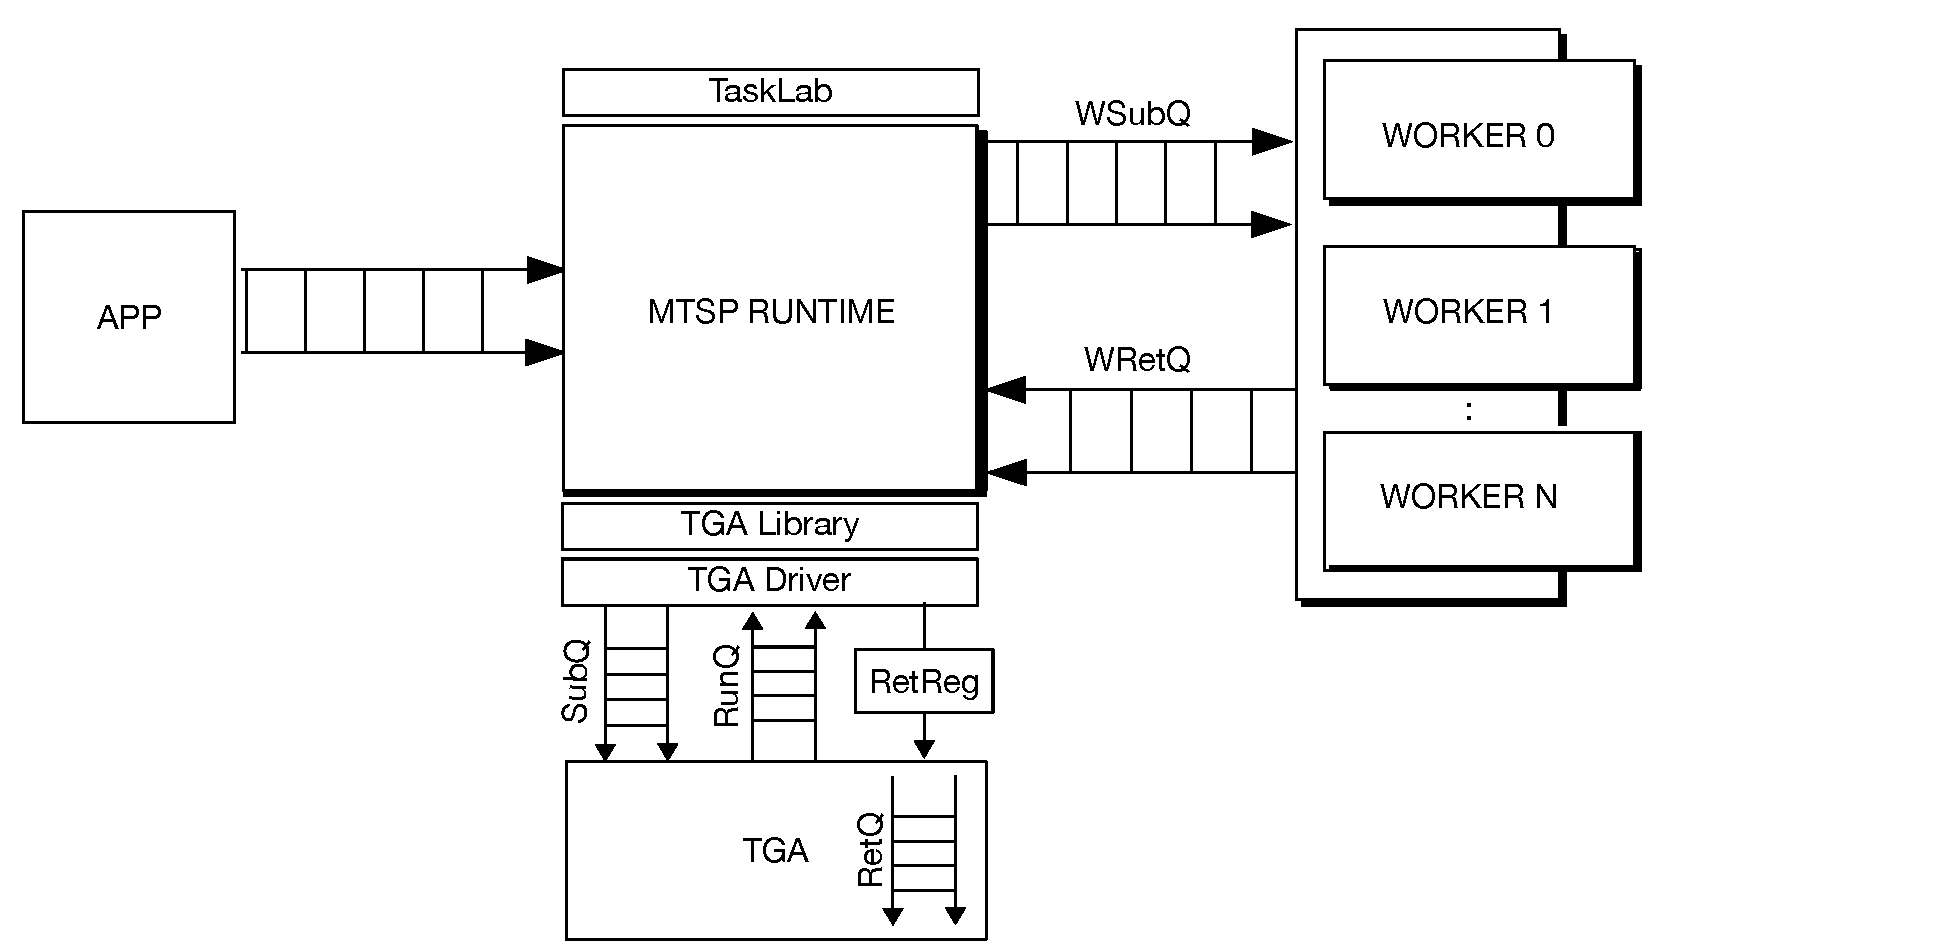
\includegraphics[width=12cm]{figures/MTSP-Driver.pdf}
  \caption{Architecture of the MTSP runtime and its interface to the TGA driver \cite{TIOGA} and hardware module. The runtime establish a communication between the runtime, driver and TGA by a Runtime-Library interface and TaskLab is able to talk to the runtime throught the upper level. }
  \label{fig:arch}
\end{figure}

\isadora{I think it needs a paragraph describing "Taquaral" (that's what I've been calling so far, for a lack of better name) and describing its functionality.
  The figure would need to be remade as well.}

\section{TaskLab API}
The following TaskLab API describes version 0.3. It consists of a header file, \textbf{TaskLab.h}, and its implementation, \textbf{TaskLab.cpp}, which contains functionality regarding: DAG generation; run task graphs in the runtime; visualization and (de)serialization of task graphs; trace from real applications.

\subsection{TaskLab data structures}
\begin{verbatim}
typedef struct task_s {
public:
    uint16_t    tID;         // hardware internal task ID
    uint64_t    WDPtr;       // address pointing to the task function
    int         ndeps;       // number of dependencies of the task
    dep*        deparr;      // list of dependencies of the task
} task;

\end{verbatim}

\begin{verbatim}
typedef struct dep_s {
    uint64_t     varptr;     // address of the dependency variable
    uint8_t      mode;       // mode of the variable 
} dep; 
\end{verbatim}

Notice that these are the structures visible to the user, which are the same from the TGA Library \cite{TIOGA}. The API, however, use different structures to handle internal data (such as \texttt{\_tasks} and \texttt{\_deps}), but its communication relies only on these structures above. 

For clarification purposes, TaskLab internal structures are defined above.

\begin{verbatim}
typedef struct dep_i {
public:
    uint32_t task;  // task that the dependency is heading towards to
    uint8_t  type;  // type of dependency
    uint32_t dID;   // index of dependency
    uint32_t var;   // var that relies on
} _dep;
\end{verbatim}

\begin{verbatim}
typedef struct task_i {
public:
    std::list<_dep> predecessors;  // predecessors tasks
    std::list<_dep> successors;    // successors tasks
    uint32_t tID;                  // index of task
    uint32_t npred;                // total number of predecessors
    float    exec;                 // how long should the task remain executing
} _task;
\end{verbatim}


\subsection{TaskLab classes}
These are the classes used by the API, which is Object-oriented. Private methods were ommited for a clearer understanding.

\begin{verbatim}
class TaskGraph {
private:
    std::vector<_task> tasks;  // tasks structure
    uint32_t  ntasks;          // total number of tasks
    uint32_t  ndeps;           // total number of dependencies between tasks
    uint32_t  nvar;            // total number of variables shared between tasks
    uint32_t  dep_r;           // max range of how far a predecessor may be
    uint32_t  exec_t;          // standard execution time per task (ms)
    float     max_r;           // max. range from standard execution time (0 to 1)

    std::map< uint64_t, std::vector<_dep> > in_map;
    std::map< uint64_t, _dep >              out_map;
}
\end{verbatim}

\begin{verbatim}
class TaskLab {
public:
    void generate(const uint32_t n, const uint32_t m,
                  const uint32_t d, const uint32_t t,
                  const float    r);
    bool run(const uint8_t rt);

    void burnin(const uint32_t nruns, const uint32_t max_t, const uint8_t rt);

    bool hasEvent(uint8_t event);
    void watchEvent(uint8_t event);
    void eventOccurred(uint8_t event, void* t);

    void save(const char* filename);
    void restore(const char* filename);
    void plot(const char* filename);

private:
    TaskGraph*          tg;

    bool                t_e[EVENT_S] {0}; // watchable trace events

    static TaskGraph*   tg_t;
    static bool         r_error;
}
\end{verbatim}

\subsection{TaskLab method descriptions}
Below is the description of \textbf{public} functions available in TaskLab.

\begin{itemize}
\item \texttt{\noindent void TaskLab::generate \newline
(const uint32\_t n, const uint32\_t m, const uint32\_t d, \newline
 const uint32\_t t, const float r)} \newline
Method responsible for generating a DAG, which represents an application with task parallelism to be simulated. The parameters required for the generation are described below; notice that all the optional parameters have a default value, which can be defined by the user.
\begin{itemize}
\item \texttt{n} is the number of tasks to be generated; 
\item \texttt{m} is the maximum number of IN/INOUT dependencies that has to be created on each task, minimum is 1 by default; 
\item \texttt{d} sets how far a predecessor may be from a parent (optional); 
\item \texttt{t} is is the standard execution time per task (ms) (optional); 
\item \texttt{r} is the maximum range from standard load time (from 0 to 1) (optional). 
\end{itemize}

\item \texttt{void TaskLab::run(const uint8\_t rt)} \newline
Dispatches a current loaded graph to the \texttt{rt} runtime, displaying on-the-fly information about tasks, and whether if the simulation ran correctly. Its success is defined by checking if the graph was executed in the appropriate order, i.e. it respected the given dependencies. TaskLab communicates with the runtime by calling functions that receives tasks and execute them. Each task calls an arbitrary function which simply awaits for the given load time.

\item \texttt{void TaskLab::burnin(const uint32\_t nruns, const uint32\_t max\_t, const uint8\_t rt)} \newline
This method is responsible for generating and dispatching to the \texttt{rt} runtime a total of \texttt{nruns} random task graphs, within a limit of \texttt{max\_t} tasks by graph. It displays output for each task graph and if the simulation ran correctly.

\item\texttt{bool TaskLab::hasEvent(const uint8\_t event)} \newline
Checks if an \texttt{event} is currently being watched by the API - if so, returns true, otherwise false.

\item\texttt{void TaskLab::watchEvent(const uint8\_t event)} \newline
Notifies API to watch an \texttt{event} from a running application, i.e. record task dispatching.

\item\texttt{void TaskLab::eventOccurred(const uint8\_t event, void* t)} \newline
Method used by the runtime in order to notify API that an event occurred, if necessary. Event is of type \texttt{event} and \texttt{t} is its content. Currently supported types are described below.
\begin{itemize} 
\item Event of type \texttt{Evt::TASK}; it receives an parameter \texttt{t} of type \texttt{task}, which is added to the task graph.
\end{itemize}

\item \texttt{void TaskLab::save(const char* filename)} \newline
Save a graph as a \textit{.dat} file, by serializing it. It takes as parameter the \texttt{filename} of the serialized graph file.

\item \texttt{void TaskLab::restore(const char* filename)} \newline
This method is responsible for retrieving a graph stored as a \textit{.dat} file, by deserializing it. It takes as parameter the \texttt{filename} of the serialized graph file.

\item \texttt{void TaskLab::plot(const char* filename)} \newline
Save a graph as a \textit{.dot} file, allowing to visualize it. It takes as parameter the corresponding \texttt{filename} of the graph.
\end{itemize}

\subsection{Task graph generation procedure}
The generation of the task graph works as follows: first, the graph is created with \texttt{n} tasks, specified by the user. For each created task: a random load time is assigned according to the \texttt{default load time} and its \texttt{maximum range} - for example, if the default load time is 1000 ms and the load range is 0.25, it may vary from 750ms to 1250ms; a random number of dependencies is created, ranging from 1 to \texttt{maximum}, also specified by the user.   Then, each dependency in the task is described as follows: a unique id is assigned, for later on purposes; a predecessor that haven't been picked yet is selected, which its \texttt{maximum distance} is defined according to the parameter of dependency range; the predecessor task receives an OUT dependency, with the same id as the successor dependency, relating both tasks; finally, the dependency is assigned as IN or INOUT, randomly. 

\subsection{Task graph validation procedure}
The execution of the graph is validated by creating a boolean list with all the dependencies of the graph based on its unique id, assigned initially to false. It consists of: when a task executes, it assigns all of its successors' dependency as true. Then, if a task executes and all of its predecessors' dependency is defined as true, it means that is safe to execute, i.e. all of its father tasks have already executed; otherwise, the execution is not correct. If every task executed correctly, it means that the graph is validated and successfully executed.

\subsection{Task tracing prodecure}
(TBD)

\section{Next Steps}
The v0.2 release of the TaskLab is currently user development. Some features that it will provide are:
 \begin{itemize}
\item Compatibility with other runtimes;
\item More customization regarding graph generation;
\item Trace capture, storage and replay of task execution. 
\end{itemize}

\bibliography{bib/tasklab} 
\bibliographystyle{ieeetr}

\end{document}
